\begin{minipage}{0.49\textwidth}
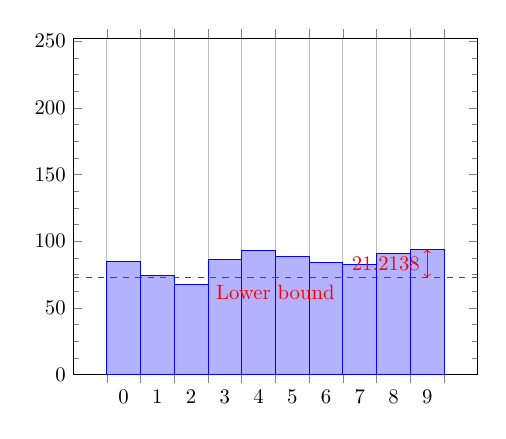
\begin{tikzpicture}[scale=0.75]
  \begin{axis}[ybar interval, ymax=252.355,ymin=0, minor y tick num = 3]
    \addplot coordinates { (0,84.7931) (1,73.9828) (2,67.7931) (3,86.1897) (4,93.0517) (5,88.7414) (6,84.069) (7,82.2931) (8,90.7414) (9,93.8621) (10, 114.707) };
\draw [red, dashed] ({rel axis cs:0,0}|-{axis cs:0,72.6483}) -- ({rel axis cs:1,0}|-{axis cs:10,72.6483}) node [pos=0.5, below] {Lower bound};
\draw [red, <->] ({axis cs:9.5,72.6483}) -- ({axis cs:9.5,93.8621}) node [pos=0.5, left] { 21.2138};
  \end{axis}
\end{tikzpicture}
\caption*{Weights repartitions on the first tree}
\end{minipage}
\begin{minipage}{0.49\textwidth}
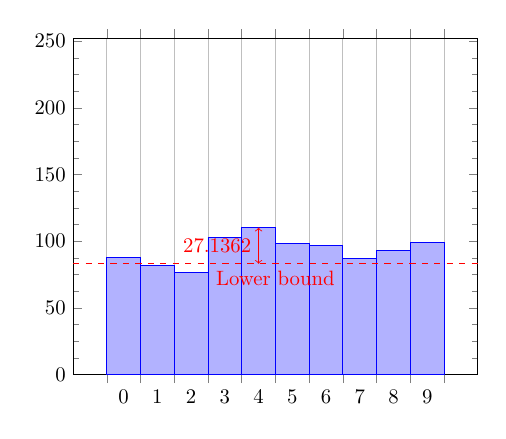
\begin{tikzpicture}[scale=0.75]
  \begin{axis}[ybar interval, ymax=252.355,ymin=0, minor y tick num = 3]
    \addplot coordinates { (0,87.931) (1,81.7931) (2,76.7759) (3,102.879) (4,110.155) (5,97.9828) (6,96.9138) (7,86.7586) (8,92.7241) (9,99.2586) (10, 114.707) };
\draw [red, dashed] ({rel axis cs:0,0}|-{axis cs:0,83.019}) -- ({rel axis cs:1,0}|-{axis cs:10,83.019}) node [pos=0.5, below] {Lower bound};
\draw [red, <->] ({axis cs:4.5,83.019}) -- ({axis cs:4.5,110.155}) node [pos=0.5, left] { 27.1362};
  \end{axis}
\end{tikzpicture}
\caption*{Weights repartitions on the last}
\end{minipage}
\begin{minipage}{0.49\textwidth}
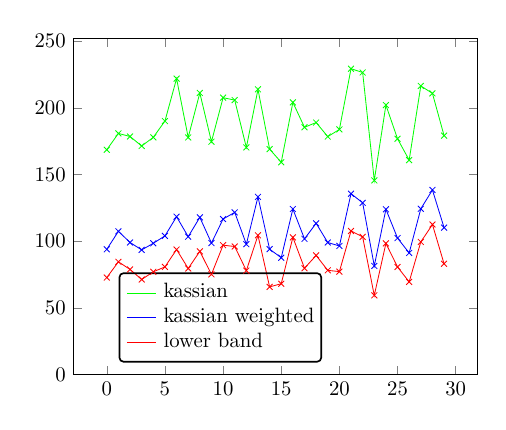
\begin{tikzpicture}[scale=0.75]
  \begin{axis}[ymax=252.355,ymin=0]
    \addplot[color=green, mark=x] coordinates { (0,168.603) (1,180.828) (2,178.534) (3,171.414) (4,177.914) (5,190.121) (6,221.966) (7,177.828) (8,211.207) (9,174.638) (10,207.672) (11,205.845) (12,170.31) (13,213.931) (14,169.052) (15,159.172) (16,204.121) (17,185.431) (18,189.017) (19,178.448) (20,183.81) (21,229.414) (22,226.569) (23,145.586) (24,202.121) (25,176.81) (26,160.828) (27,216.466) (28,210.931) (29,179.207) };
    \addplot[color=blue, mark=x] coordinates { (0,93.8621) (1,107.379) (2,98.9828) (3,93.431) (4,98.3793) (5,103.948) (6,118.328) (7,103.362) (8,117.845) (9,98.5517) (10,116.603) (11,121.569) (12,97.6897) (13,133.224) (14,93.9655) (15,87.5862) (16,124.121) (17,101.707) (18,113.379) (19,98.9655) (20,96.3793) (21,135.603) (22,128.776) (23,81.4138) (24,123.914) (25,102.276) (26,91.1552) (27,124.259) (28,138.414) (29,110.155) };
    \addplot[color=red, mark=x] coordinates { (0,72.6483) (1,84.4931) (2,78.7741) (3,71.2121) (4,76.9862) (5,80.6603) (6,93.6862) (7,79.4845) (8,92.3224) (9,75.0724) (10,96.9586) (11,95.9638) (12,77.9172) (13,104.364) (14,65.6707) (15,68.031) (16,102.85) (17,79.6879) (18,89.2552) (19,78.0862) (20,77.1207) (21,107.645) (22,103.197) (23,59.3052) (24,98.3017) (25,80.5966) (26,69.4362) (27,99.419) (28,112.484) (29,83.019) };
\node[draw=black,thick,rounded corners=2pt,above right=2mm] at (0, 0) {%
  \begin{tabular}{@{}r@{ }l@{}}
    \raisebox{2pt}{\tikz{\draw[green] (0,0) -- (5mm,0);}}&kassian\\
    \raisebox{2pt}{\tikz{\draw[blue] (0,0) -- (5mm,0);}}&kassian weighted\\
    \raisebox{2pt}{\tikz{\draw[red] (0,0) -- (5mm,0);}}&lower band
  \end{tabular}};
\end{axis}
\end{tikzpicture}
\caption*{ Per tree, maximum weights with kassian and our algorithm, and lower band }
\end{minipage}
